%        File: arfc-beamer.tex
%     Created: Sun May 5 10:00 PM 2013 C
%


%\documentclass[11pt,handout]{beamer}
\documentclass[9pt]{beamer}
\usetheme[white]{Illinois}
%\title[short title]{long title}
\title[Osier for Fuel Cycles]{\Acrlong{osier} for fuel cycle analysis and optimization}
%\subtitle[short subtitle]{long subtitle}
% \subtitle[Short SubTitle]{Mostly Kittens}
%\author[short name]{long name}
\author[Samuel Dotson]{Samuel Dotson\\Advanced Reactors and Fuel Cycles Group}
%\date[short date]{long date}
\date[06.12.2025]{June 12, 2025}
%\institution[short name]{long name}
\institute[UIUC]{University of Illinois Urbana-Champaign}

%\usepackage{bbding}
\usepackage{amsfonts}
\usepackage{amsmath}
\usepackage{xspace}
\usepackage{graphicx}
\usepackage{subfigure}
\usepackage{booktabs} % nice rules for tables
\usepackage{microtype} % if using PDF
\usepackage{bigints}
\usepackage{minted}

\newcommand{\units}[1] {\:\text{#1}}%
\newcommand{\SN}{S$_N$}%{S$_\text{N}$}%{$S_N$}%
\DeclareMathOperator{\erf}{erf}
%I need some complimentary error functions...
\DeclareMathOperator{\erfc}{erfc}
%Those icons in the references are terrible looking
\setbeamertemplate{bibliography item}[text]

%%%% Acronym support

\usepackage[acronym,toc]{glossaries}
%\newacronym{<++>}{<++>}{<++>}
\newacronym[longplural={metric tons of heavy metal}]{MTHM}{MTHM}{metric ton of heavy metal}
\newacronym{ABM}{ABM}{agent-based modeling}
\newacronym{ACDIS}{ACDIS}{Program in Arms Control \& Domestic and International Security}
\newacronym{ADS}{ADS}{Accelerator-Driven Systems}
\newacronym{AHTR}{AHTR}{Advanced High Temperature Reactor}
\newacronym{ANDRA}{ANDRA}{Agence Nationale pour la gestion des D\'echets RAdioactifs, the French National Agency for Radioactive Waste Management}
\newacronym{ANL}{ANL}{Argonne National Laboratory}
\newacronym{ANS}{ANS}{American Nuclear Society}
\newacronym{API}{API}{application programming interface}
\newacronym{ARE}{ARE}{Aircraft Reactor Experiment}
\newacronym{ARFC}{ARFC}{Advanced Reactors and Fuel Cycles}
\newacronym{ASME}{ASME}{American Society of Mechanical Engineers}
\newacronym{ASTRID}{ASTRID}{Advanced Sodium Technological Reactor for Industrial Demonstration}
\newacronym{ATWS}{ATWS}{Anticipated Transient Without Scram}
\newacronym{BDBE}{BDBE}{Beyond Design Basis Event}
\newacronym{BIDS}{BIDS}{Berkeley Institute for Data Science}
\newacronym{BWR}{BWR}{Boiling Water Reactor}
\newacronym{CAFCA}{CAFCA}{ Code for Advanced Fuel Cycles Assessment }
\newacronym{CDTN}{CDTN}{Centro de Desenvolvimento da Tecnologia Nuclear}
\newacronym{CEA}{CEA}{Commissariat \`a l'\'Energie Atomique et aux \'Energies Alternatives}
\newacronym{CI}{CI}{continuous integration}
\newacronym{CNEN}{CNEN}{Comiss\~{a}o Nacional de Energia Nuclear}
\newacronym{CNERG}{CNERG}{Computational Nuclear Engineering Research Group}
\newacronym{COSI}{COSI}{Commelini-Sicard}
\newacronym{COTS}{COTS}{commercial, off-the-shelf}
\newacronym{CSNF}{CSNF}{commercial spent nuclear fuel}
\newacronym{CTAH}{CTAHs}{Coiled Tube Air Heaters}
\newacronym{CUBIT}{CUBIT}{CUBIT Geometry and Mesh Generation Toolkit}
\newacronym{CURIE}{CURIE}{Centralized Used Fuel Resource for Information Exchange}
\newacronym{DAG}{DAG}{directed acyclic graph}
\newacronym{DANESS}{DANESS}{Dynamic Analysis of Nuclear Energy System Strategies}
\newacronym{DBE}{DBE}{Design Basis Event}
\newacronym{DESAE}{DESAE}{Dynamic Analysis of Nuclear Energy Systems Strategies}
\newacronym{DHS}{DHS}{Department of Homeland Security}
\newacronym{DOE}{DOE}{Department of Energy}
\newacronym{DRACS}{DRACS}{Direct Reactor Auxiliary Cooling System}
\newacronym{DRE}{DRE}{dynamic resource exchange}
\newacronym{DSNF}{DSNF}{DOE spent nuclear fuel}
\newacronym{DYMOND}{DYMOND}{Dynamic Model of Nuclear Development }
\newacronym{EBS}{EBS}{Engineered Barrier System}
\newacronym{EDF}{EDF}{Électricité de France}
\newacronym{EDZ}{EDZ}{Excavation Disturbed Zone}
\newacronym{EIA}{EIA}{U.S. Energy Information Administration}
\newacronym{EPA}{EPA}{Environmental Protection Agency}
\newacronym{EPR}{EPR}{European Pressurized Reactor}
\newacronym{EP}{EP}{Engineering Physics}
\newacronym{EU}{EU}{European Union}
\newacronym{FCO}{FCO}{Fuel Cycle Options}
\newacronym{FCT}{FCT}{Fuel Cycle Technology}
\newacronym{FEHM}{FEHM}{Finite Element Heat and Mass Transfer}
\newacronym{FEPs}{FEPs}{Features, Events, and Processes}
\newacronym{FHR}{FHR}{Fluoride-Salt-Cooled High-Temperature Reactor}
\newacronym{FLiBe}{FLiBe}{Fluoride-Lithium-Beryllium}
\newacronym{FP}{FP}{Fission Products}
\newacronym{GDSE}{GDSE}{Generic Disposal System Environment}
\newacronym{GDSM}{GDSM}{Generic Disposal System Model}
\newacronym{GENIUSv1}{GENIUSv1}{Global Evaluation of Nuclear Infrastructure Utilization Scenarios, Version 1}
\newacronym{GENIUSv2}{GENIUSv2}{Global Evaluation of Nuclear Infrastructure Utilization Scenarios, Version 2}
\newacronym{GENIUS}{GENIUS}{Global Evaluation of Nuclear Infrastructure Utilization Scenarios}
\newacronym{GPAM}{GPAM}{Generic Performance Assessment Model}
\newacronym{GRSAC}{GRSAC}{Graphite Reactor Severe Accident Code}
\newacronym{GUI}{GUI}{graphical user interface}
\newacronym{HLW}{HLW}{high level waste}
\newacronym{HPC}{HPC}{high-performance computing}
\newacronym{HTC}{HTC}{high-throughput computing}
\newacronym{HTGR}{HTGR}{High Temperature Gas-Cooled Reactor}
\newacronym{IAEA}{IAEA}{International Atomic Energy Agency}
\newacronym{IEMA}{IEMA}{Illinois Emergency Mangament Agency}
\newacronym{IHLRWM}{IHLRWM}{International High Level Radioactive Waste Management}
\newacronym{INL}{INL}{Idaho National Laboratory}
\newacronym{IPRR1}{IRP-R1}{Instituto de Pesquisas Radioativas Reator 1}
\newacronym{IRP}{IRP}{Integrated Research Project}
\newacronym{ISFSI}{ISFSI}{Independent Spent Fuel Storage Installation}
\newacronym{ISRG}{ISRG}{Independent Student Research Group}
\newacronym{JFNK}{JFNK}{Jacobian-Free Newton Krylov}
\newacronym{LANL}{LANL}{Los Alamos National Laboratory}
\newacronym{LBNL}{LBNL}{Lawrence Berkeley National Laboratory}
\newacronym{LCOE}{LCOE}{levelized cost of electricity}
\newacronym{LDRD}{LDRD}{laboratory directed research and development}
\newacronym{LFR}{LFR}{Lead-Cooled Fast Reactor}
\newacronym{LLNL}{LLNL}{Lawrence Livermore National Laboratory}
\newacronym{LMFBR}{LMFBR}{Liquid Metal Fast Breeder Reactor}
\newacronym{LOFC}{LOFC}{Loss of Forced Cooling}
\newacronym{LOHS}{LOHS}{Loss of Heat Sink}
\newacronym{LOLA}{LOLA}{Loss of Large Area}
\newacronym{LP}{LP}{linear program}
\newacronym{LWR}{LWR}{Light Water Reactor}
\newacronym{MAGNOX}{MAGNOX}{Magnesium Alloy Graphie Moderated Gas Cooled Uranium Oxide Reactor}
\newacronym{MA}{MA}{minor actinide}
\newacronym{MCNP}{MCNP}{Monte Carlo N-Particle code}
\newacronym{MILP}{MILP}{mixed-integer linear program}
\newacronym{MIT}{MIT}{the Massachusetts Institute of Technology}
\newacronym{MOAB}{MOAB}{Mesh-Oriented datABase}
\newacronym{MOOSE}{MOOSE}{Multiphysics Object-Oriented Simulation Environment}
\newacronym{MOX}{MOX}{Mixed Oxide Fuel}
\newacronym{MSBR}{MSBR}{Molten Salt Breeder Reactor}
\newacronym{MSRE}{MSRE}{Molten Salt Reactor Experiment}
\newacronym{MSR}{MSR}{Molten Salt Reactor}
\newacronym{NAGRA}{NAGRA}{National Cooperative for the Disposal of Radioactive Waste}
\newacronym{NEAMS}{NEAMS}{Nuclear Engineering Advanced Modeling and Simulation}
\newacronym{NEUP}{NEUP}{Nuclear Energy University Programs}
\newacronym{NFCSim}{NFCSim}{Nuclear Fuel Cycle Simulator}
\newacronym{NGNP}{NGNP}{Next Generation Nuclear Plant}
\newacronym{NMWPC}{NMWPC}{Nuclear MW Per Capita}
\newacronym{NNSA}{NNSA}{National Nuclear Security Administration}
\newacronym{NPRE}{NPRE}{Department of Nuclear, Plasma, and Radiological Engineering}
\newacronym{NQA1}{NQA-1}{Nuclear Quality Assurance - 1}
\newacronym{NRC}{NRC}{Nuclear Regulatory Commission}
\newacronym{NSF}{NSF}{National Science Foundation}
\newacronym{NSSC}{NSSC}{Nuclear Science and Security Consortium}
\newacronym{NUWASTE}{NUWASTE}{Nuclear Waste Assessment System for Technical Evaluation}
\newacronym{NWF}{NWF}{Nuclear Waste Fund}
\newacronym{NWTRB}{NWTRB}{Nuclear Waste Technical Review Board}
\newacronym{OCRWM}{OCRWM}{Office of Civilian Radioactive Waste Management}
\newacronym{ORION}{ORION}{ORION}
\newacronym{ORNL}{ORNL}{Oak Ridge National Laboratory}
\newacronym{PARCS}{PARCS}{Purdue Advanced Reactor Core Simulator}
\newacronym{PBAHTR}{PB-AHTR}{Pebble Bed Advanced High Temperature Reactor}
\newacronym{PBFHR}{PB-FHR}{Pebble-Bed Fluoride-Salt-Cooled High-Temperature Reactor}
\newacronym{PEI}{PEI}{Peak Environmental Impact}
\newacronym{PH}{PRONGHORN}{PRONGHORN}
\newacronym{PRIS}{PRIS}{Power Reactor Information System}
\newacronym{PRKE}{PRKE}{Point Reactor Kinetics Equations}
\newacronym{PSPG}{PSPG}{Pressure-Stabilizing/Petrov-Galerkin}
\newacronym{PWAR}{PWAR}{Pratt and Whitney Aircraft Reactor}
\newacronym{PWR}{PWR}{Pressurized Water Reactor}
\newacronym{PyNE}{PyNE}{Python toolkit for Nuclear Engineering}
\newacronym{PyRK}{PyRK}{Python for Reactor Kinetics}
\newacronym{QA}{QA}{quality assurance}
\newacronym{RDD}{RD\&D}{Research Development and Demonstration}
\newacronym{RD}{R\&D}{Research and Development}
\newacronym{RELAP}{RELAP}{Reactor Excursion and Leak Analysis Program}
\newacronym{RIA}{RIA}{Reactivity Insertion Accident}
\newacronym{RIF}{RIF}{Region-Institution-Facility}
\newacronym{SFR}{SFR}{Sodium-Cooled Fast Reactor}
\newacronym{SINDAG}{SINDA{\textbackslash}G}{Systems Improved Numerical Differencing Analyzer $\backslash$ Gaski}
\newacronym{SKB}{SKB}{Svensk K\"{a}rnbr\"{a}nslehantering AB}
\newacronym{SNF}{SNF}{spent nuclear fuel}
\newacronym{SNL}{SNL}{Sandia National Laboratory}
\newacronym{STC}{STC}{specific temperature change}
\newacronym{SUPG}{SUPG}{Streamline-Upwind/Petrov-Galerkin}
\newacronym{SWF}{SWF}{Separations and Waste Forms}
\newacronym{SWU}{SWU}{Separative Work Unit}
\newacronym{TRIGA}{TRIGA}{Training Research Isotope General Atomic}
\newacronym{TRISO}{TRISO}{Tristructural Isotropic}
\newacronym{TSM}{TSM}{Total System Model}
\newacronym{TSPA}{TSPA}{Total System Performance Assessment for the Yucca Mountain License Application}
\newacronym{ThOX}{ThOX}{thorium oxide}
\newacronym{UFD}{UFD}{Used Fuel Disposition}
\newacronym{UML}{UML}{Unified Modeling Language}
\newacronym{UNF}{UNF}{Used Nuclear Fuel}
\newacronym{UOX}{UOX}{Uranium Oxide Fuel}
\newacronym{UQ}{UQ}{uncertainty quantification}
\newacronym{US}{US}{United States}
\newacronym{UW}{UW}{University of Wisconsin}
\newacronym{VISION}{VISION}{the Verifiable Fuel Cycle Simulation Model}
\newacronym{VVER}{VVER}{Voda-Vodyanoi Energetichesky Reaktor (Russian Pressurized Water Reactor)}
\newacronym{VV}{V\&V}{verification and validation}
\newacronym{WIPP}{WIPP}{Waste Isolation Pilot Plant}
\newacronym{YMR}{YMR}{Yucca Mountain Repository Site}


% \makeglossaries

%try to get rid of header on title page\dots
\makeatletter
    \newenvironment{withoutheadline}{
        \setbeamertemplate{headline}[default]
        \def\beamer@entrycode{\vspace*{-\headheight}}
    }{}
\makeatother

\makeatother
\setbeamertemplate{footline}
{
  \leavevmode%
  \hbox{%
    \rightline{\insertframenumber{} / \inserttotalframenumber\hspace*{1ex}}
  }%
  \vskip0pt%
}
\makeatletter
% This will add figure numbers to captions.
\setbeamertemplate{caption}[numbered]

\begin{document}
%%%%%%%%%%%%%%%%%%%%%%%%%%%%%%%%%%%%%%%%%%%%%%%%%%%%%%%%%%%%%
%% From uw-beamer Here's a handy bit of code to place at
%% the beginning of your presentation (after \begin{document}):
\newcommand*{\alphabet}{ABCDEFGHIJKLMNOPQRSTUVWXYZabcdefghijklmnopqrstuvwxyz}
\newlength{\highlightheight}
\newlength{\highlightdepth}
\newlength{\highlightmargin}
\setlength{\highlightmargin}{2pt}
\settoheight{\highlightheight}{\alphabet}
\settodepth{\highlightdepth}{\alphabet}
\addtolength{\highlightheight}{\highlightmargin}
\addtolength{\highlightdepth}{\highlightmargin}
\addtolength{\highlightheight}{\highlightdepth}
\newcommand*{\Highlight}{\rlap{\textcolor{HighlightBackground}{\rule[-\highlightdepth]{\linewidth}{\highlightheight}}}}
%%%%%%%%%%%%%%%%%%%%%%%%%%%%%%%%%%%%%%%%%%%%%%%%%%%%%%%%%%%%%
%%--------------------------------%%
\begin{withoutheadline}
\frame{
  \titlepage
}
\end{withoutheadline}

%%--------------------------------%%
\AtBeginSection[]{
\begin{frame}
  \frametitle{Outline}
  \tableofcontents[currentsection]
\end{frame}
}

\section{Motivation}
% \subsection{Cat Behavior}
% \begin{frame}
  \frametitle{An Image}
  % a comment
  \begin{figure}[htbp!]
    \begin{center}
      
\includegraphics[height=4cm]{./images/kitten}
    \end{center}
          \caption{A caption describing the image. \cite{lastname_firstword_1900}.}
    \label{fig:kittenfigure}
  \end{figure}
\end{frame}

\begin{frame}
  \frametitle{A Table}
        Frames (slides) can have ``blocks.'' 
        \begin{block}{This one is about a cat}
                A cat in a hat.
        \end{block}
        \begin{block}{A cat}
                In a hat.

                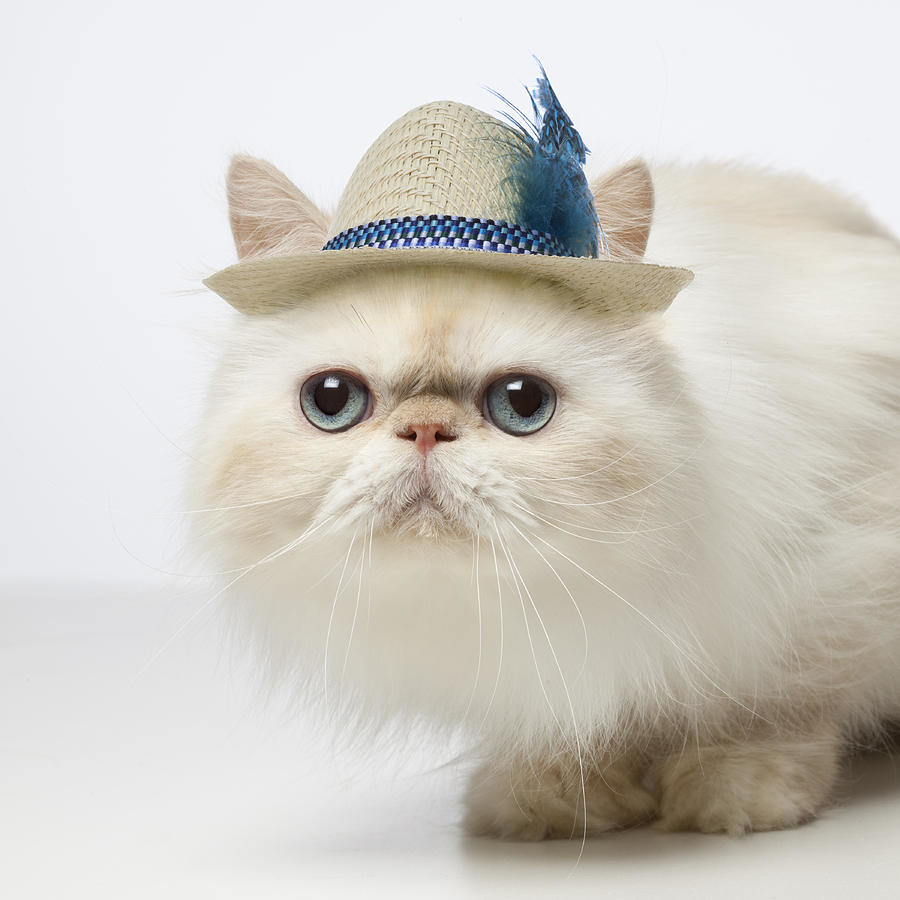
\includegraphics[height=0.2\textheight]{./images/catinhat}
        \end{block}
        
\end{frame}

% \subsection{Cat Appearance}
% \begin{frame}
  \frametitle{Columns}
  % a comment
        \begin{columns}
                \column[t]{5cm}
                Sometimes things need to be put side by side, in two nice 
                looking columns. 

                Maybe one column involves a quotation.

                \begin{quote}
                        Explicit is better than implicit. -- The Zen of Python
                \end{quote}


                And, also, perhaps, a logo.
                \begin{center}
                        
\includegraphics[height=0.2\textheight]{./images/arfc-logo}
                \end{center}
                \column[t]{5cm}
        \begin{figure}[htbp!]
        \begin{center}
      
\includegraphics[height=4cm]{./images/kitten}
    \end{center}
          \caption{A caption describing the image. \cite{lastname_firstword_1900}.}
    \label{fig:kittenfigure}
  \end{figure}
        \end{columns}
\end{frame}

\begin{frame}[fragile]
  \frametitle{Some Code}
        I have to use the fragile syntax for code slides.
        \begin{minted}{python}
def meow(volume):
    """Make a demanding noise at the specified volume
    
    Parameters
    ----------
    volume: int
        The volume of the demand. No relation to importance.

    Returns
    -------
    str
        meow
    """
    o = 'o'*volume
    return 'me'+ o + 'ow'
\end{minted}
\end{frame}

% \subsection{Cat Math}
% \begin{frame}
  \frametitle{Cat Math: Part 1}
  % a comment
        \begin{align}
                x &= y
                \intertext{where}
                x &= \mbox{cats}\\
                y &= \mbox{peculiar}
        \end{align}
\end{frame}

\begin{frame}
\frametitle{Cat Math: Part 2}
        Everything in Beamer is just like in \LaTeX.
        Right down to the theorems.
        \begin{theorem}[Pythagoras] 
                $ a^2 + b^2 = c^2$
        \end{theorem}
        \begin{corollary}
                $ x + y = y + x  $
        \end{corollary}
        \begin{proof}
                $\omega +\phi = \epsilon $
        \end{proof}


\end{frame}

\section{Pareto Optimality}
% \section{\Gls{osier}}
\section{\Gls{set}}
\section{Results}
\section{Results}

\subsection{Nuclear Material Inventory}

\Cref{tab:sim_result1} lists \gls{EU} material inventory in 2050.

\begin{table}[h]
	\centering
%	\scalebox{0.86}{
		\begin{tabular}{cccc}
			\hline
			\textbf{Category } & \textbf{Value} & \textbf{Unit} & \textbf{Specifics}\\ \hline
			UOX Usage  & 158,794 & MTHM &  \\ 
			MOX Usage  & 6,671 & MTHM & \\ 
			\textbf{Used UOX Stored}  & \textbf{95,161} & MTHM & \gls{UNF} that is not reprocessed\\
			\textbf{Used UOX Stored (France)} & \textbf{9,979} & MTHM & \gls{UNF} that is not reprocessed \\
			Tails  & 979,463 & MTHM & \\ 
			Natural U Used  & 1,141,916 & MTHM & \\ \hline
		\end{tabular}
		\caption{Nuclear material inventory in the \gls{EU} in 2050 is summarized. 
				 The difference between total \gls{UOX} usage and \gls{UOX} stored is the amount
				 that has been reprocessed for \gls{MOX}. Only the stored \gls{UOX} is used for \gls{ASTRID} fuel production.}
		\label{tab:sim_result1}
\end {table}
\FloatBarrier


Figures \ref{fig:eu_tail} and \ref{fig:eu_snf} show the 
accumulation of tails and used fuel over time in \gls{EU}.
Tails accumulate as a by-product of uranium enrichment. For every
ton of \gls{UOX} fuel, about nine times of tails is produced. 
Spent fuel is discharged from reactors every refueling period.
The entire core is discharged when the reactor decommissions.
A total of about $1,000,000 MTHM$ of tails and $100,000 MTHM$ of
\gls{UNF} accumulate in 2050.
Figure \ref{fig:eu_fuel} shows the amount of fuel used in \gls{EU}.


\begin{figure}[htbp!]
	\begin{center}
		\includegraphics[scale=0.7]{./images/eu_future/tails.png}
	\end{center}
	\caption{This plot shows the timeseries of tails mass accumulation and discharge in the \gls{EU} nations.
			 Tails mass accumulation is fairly steady, with peaks occurring when
			 new reactors are deployed.}
	\label{fig:eu_tail}
\end{figure}

\begin{figure}[htbp!]
	\begin{center}
		\includegraphics[scale=0.7]{./images/eu_future/total_fuel.png}
	\end{center}
	\caption{This plot shows the timeseries of total fuel usage in the \gls{EU} nations.}
	\label{fig:eu_fuel}
\end{figure}


\begin{figure}[htbp!]
	\begin{center}
			\includegraphics[scale=0.7]{./images/eu_future/snf_discharge.png}
	\end{center}
	\caption{This plot displays the timeseries of \gls{UNF} accumulation and discharge in the \gls{EU} nations.
			 The peaks are caused by decommissioning of reactors, where all the core is sent to the repository.}
	\label{fig:eu_snf}
\end{figure}
\FloatBarrier


\begin{table}[h]
	\centering
	\begin{tabular}{ccc}
		\hline
		\textbf{Isotope} & \textbf{Mass Fraction in Used Fuel [\%]} & \textbf{Quantity [t]} \\ \hline
		Pu238 & 0.0111 & 10.5628 \\ 
		Pu239 & 0.518 & 492.93 \\ 
		Pu240 & 0.232 & 220.7 \\ 
		Pu241 & 0.126 & 119.9 \\ 
		Pu242 & 0.0487 & 46.3 \\ \hline
		\textbf{Total} & \textbf{0.9358} & \textbf{890.5} \\ \hline
	\end{tabular}
	\caption{Plutonium From \gls{UNF} Inventory. This table assumes no decay
			 took place. The long half-life of the fissile Pu-239 (24,100 years)
			 weakens the impact of decay on the usability of \gls{UNF}.}
	\label{tab:pu}
\end{table}


\Cref{tab:pu} lists the isotope, mass fraction,
and quantity of plutonium that can be obtained from the 2050 \gls{UNF} inventory.


\subsection{French \gls{SFR} Deployment}

Reprocessing \gls{UNF} collected from all EU nations can start approximately
180 \glspl{SFR}. With the \gls{SFR} breeding ratio of over one, France can transition into
a fully \gls{SFR} fleet without extra construction of \glspl{LWR}. 

From Varaine et al. \cite{varaine_pre-conceptual_2012}, a French
ASTRID-type \gls{SFR} of capacity 600 \gls{MWe} needs $1.225$ tons of
plutonium a year, with an initial plutonium loading of $4.9$ tons. 
Thus, the number of \glspl{SFR} that can be loaded with the reprocessed
plutonium from \gls{UNF} can be estimated to $\frac{Pu \ from \ legacy \ \gls{UNF}}{4.9} \approx 181$ \glspl{SFR},
assuming infinite reprocessing and fabrication capacity as well as
abundant depleted uranium supply. 

Also, assuming that \gls{MOX} can be recycled indefinitely,
used \gls{MOX} from an ASTRID reactor contains enough plutonium to produce a \gls{MOX} fuel with
the same mass, if mixed with depleted uranium. For example,
used \gls{MOX} from an ASTRID reactor is assumed to be 23.95\% plutonium
in this simulation (see \cref{tab:comp}), whereas a fresh \gls{MOX} is 22\% plutonium.
Separating plutonium from used \gls{MOX} from
an ASTRID reactor can create \gls{MOX} of the mass of used \gls{MOX}.
The plutonium breeding ratio in this simulation is thus assumed to be
$\approx 1.08$.

\Cref{fig:fuel} shows \gls{MOX} loaded in the \glspl{SFR} per month.
The spikes are due to initial fuel demand for new deployment of \glspl{SFR}.
The initial loading of new \glspl{SFR} are done with the \gls{MOX} created
from legacy \gls{UNF}. Once the deployed \glspl{SFR} create enough amounts
 of extra plutonium, the legacy \gls{UNF} is no longer used. 

\begin{figure}[htbp!]
	\begin{center}
		\includegraphics[scale=0.7]{./images/french-transition/where_fuel.png}
	\end{center}
	\caption{This plot shows the timeseries of fuel loaded into \glspl{SFR}.
			 The plot has peaks during a period of aggressive deployment of \glspl{SFR}
			 followed by an equilibrium at 150 \gls{MTHM}. The peaks reoccur with the
			 deployment of the second generation of \glspl{SFR}.}
	\label{fig:fuel}
\end{figure}
 \Cref{fig:pu_no_cum} shows the separated plutonium discharge
per month from the reprocessing plant. The plutonium outflux
does not precisely follow the fuel demand because \Cyclus agents have
material buffers that store commodity fuel for later usage. The reprocessed
plutonium from legacy \gls{UNF} is stored for the initial loading of \glspl{SFR}.
\Cref{tab:sfr_sim_result} lists metrics obtained from the second simulation.

\begin{figure}[htbp!]
	\begin{center}
		\includegraphics[scale=0.7]{./images/french-transition/pu.png}
	\end{center}
	\caption{This plot shows the separated plutonium discharge from the reprocessing plant.
			 The reprocessing demand for the first aggressive deployment of \glspl{SFR}
			 are lessened because the plutonium demand is met with plutonium separated from legacy \gls{UNF}.
			 The plutonium from reprocessing legacy fuel is a flat rectangle because the 
			 reprocessing throughput was set to 20 $\frac{tons}{month}$ to avoid reprocessing
			 all the legacy in one timestep. }
	\label{fig:pu_no_cum}
\end{figure}

\begin{table}[h]
	\centering
	\scalebox{0.86}{
		\begin{tabular}{ccc}
			\hline
			\textbf{Category} & \textbf{Unit} & \textbf{Value}  \\ \hline
			Total MOX used & MTHM & 63,820  \\ 
			\textbf{Average UOX Reprocessing} & MTHM/month & \textbf{118.92} \\
			\textbf{Average Total Reprocessing} & MTHM/month & \textbf{73.27} \\
			\textbf{Average Fuel Fabrication} & MTHM/month & \textbf{45.2} \\
			Total \glspl{SFR} Deployed & & 220 \\ 
			Total Plutonium Reprocessed & MTHM & 15,099 \\ 
			Total \gls{ASTRID} fuel from UOX Waste & MTHM & 2,923  \\ 
			Total \gls{ASTRID} fuel from MOX Waste & MTHM  & 60,535 \\ 
			Total Tails used & MTHM & 49,779 \\ 
			\textbf{Total legacy UNF reprocessed} & MTHM & \textbf{54,111} \\ 
			Total Reprocessed Uranium Stockpile & MTHM & 183,740 \\ 
			Total Raffinate & MTHM & 33,806 \\ \hline
		\end{tabular}}
		\caption {Listed are the metrics from the French transition to \gls{SFR} scenario.
				  The total legacy \gls{UNF} reprocessed is the amount of \gls{UNF} France would need
				  for a transition into a fully \gls{SFR} fleet. The tails used is around ninth
				  of the original tails inventory from the previous simulation.}
		\label{tab:sfr_sim_result}
\end {table}

Despite the large amount of initial plutonium that has to be reprocessed
prior to \gls{ASTRID} deployment, the 20 years of preparation of
\gls{ASTRID} fuel (2020-2040) allows a reasonable level of average
\gls{UOX} reprocessing capacity demand. \gls{UOX} reprocessing continues 
until 2057, when the \gls{ASTRID} spent fuel can supply the plutonium
for its own fuel.



% \section{Coupling \gls{osier} and Cyclus}
\section{Conclusion}

This work demonstrates that France can transition into
a fully \gls{SFR} fleet with installed capacity of 66,000 \gls{MWe} without
building additional \glspl{LWR}
if France receives \gls{UNF} from other \gls{EU} nations.
Supporting the \gls{SFR} fleet requires an average 
reprocessing capacity of 63.23 \gls{MTHM} per month,
and an average fabrication capacity of 45.32 \gls{MTHM} per month.

The sensitivity study explored the effect of increased \gls{SFR} breeding
ratio and existing \gls{LWR} lifetime extension. Increasing the breeding
ratio reduced the amount of \gls{LWR} \gls{UNF} required to transition
up to $9.7\%$ and decreased the total reprocessing demand up to $3.4\%$.
Increasing the lifetime of existing \glspl{LWR} was not significant
in reducing reprocessing demand, but provided the benefit of delayed
transition.

Since most \gls{EU} nations do not have an operating \gls{UNF}
repository or a management plan, they have a strong incentive
to send their \gls{UNF} to France. In particular, the nations
planning aggressive nuclear reduction will be able phase out nuclear
without constructing a permanent repository. France has an
incentive to take this fuel, since recycling used fuel from
other nations will allow France to meet their MOX demand
without new construction of \glspl{LWR}.

Table \ref{tab:which_send} lists \gls{EU} nations and their \gls{UNF} inventory
in 2050. We analyzed a strategy in which 
the nations reducing their nuclear fleet send their \gls{UNF} to France.
The sum of \gls{UNF} from Italy, Slovenia, Belgium, Spain and Germany
provides enough \gls{UNF} for the simulated transition ($\approx 53,000$ MTHM). 
These nations are shown in bold in table \ref{tab:which_send}.
Sweden is not considered because of its concrete waste management plan.

If France receives \gls{LWR} \gls{UNF} from all \gls{EU} nations,
except Sweden and Finland,
it will have a surplus of $30,648$ MTHM of \gls{LWR} \gls{UNF}. This
inventory can be leveraged to increase nuclear power capacity as
the transition takes place. However, pragmatic limitations such
as new reactor construction, reprocessing throughput, and
political concerns remain.

\begin{table}[h]
    \centering
    \caption {\gls{EU} nations and their respective \gls{UNF} inventory.} 
                \begin{tabularx}{\textwidth}{llr}
                    \hline 
                    \textbf{Nation} & \textbf{Growth Trajectory} & \small{\textbf{UNF in 2050 [MTHM] }}\\
                    \hline
                    Poland & Aggressive Growth & 1,807\\
                    Hungary & Aggressive Growth & 3,119 \\ 
                    UK & Aggressive Growth & 13,268\\
                    Slovakia & Modest Growth & 2,746\\
                    Bulgaria & Modest Growth & 3,237 \\
                    Czech Rep. & Modest Growth & 4,413\\
                    Finland & Modest Growth &  5,713\\
                    Netherlands & Modest Reduction & 539\\
                    \textbf{Italy} & \textbf{Modest Reduction} & \textbf{583}\\
                    \textbf{Slovenia} & \textbf{Modest Reduction} & \textbf{765}\\\
                    Lithuania & Modest Reduction & 2,644 \\
                    \textbf{Belgium} & \textbf{Aggressive Reduction} & \textbf{6,644}\\
                    \textbf{Spain} & \textbf{Modest Reduction} &  \textbf{9,771} \\
                    \textbf{France} & \textbf{Modest Reduction} & \textbf{12,494} \\
                    Sweden & Aggressive Reduction & 16,035\\
                    \textbf{Germany} & \textbf{Aggressive Reduction} & \textbf{23,868}\\
                    \hline
                \end{tabularx}
    
    \label{tab:which_send}

\end{table}

On the other hand, in these simulations, some complex political and economic factors were not incorporated and various assumptions were present in this scenario. For
example, Germany's current policy is to not reprocess its \gls{LWR} fuel
\cite{topfer_germanys_2011}, and this policy would create a shortage
in the supply of \gls{LWR} \gls{UNF} for \gls{ASTRID} \gls{MOX} production.
Continuation of that German policy would not, however, be incompatible
with a change in \gls{EU} policy that frees \gls{EU} countries from
creating their high level waste repositories, since France could still
agree to take in Germany's \gls{UNF} for direct disposal. The analysis
method described herein could readily be adapted to account for such possibilities. 
The collaborative option explored here may hold value for the \gls{EU} nuclear community,
and may enable France to advance more rapidly into a closed fuel cycle. 
\FloatBarrier


\section{Future Work}

Numerous assumptions for reactor physics and depletion
have been made for this work. Future work includes implementation of
a more physics-based depletion model for reactors that
can take into account the plutonium vector changes in  \gls{ASTRID} and \gls{MOX} \gls{PWR} cores.
Also, improvements can be made on incorporating enrichment differences in the initial core
batches as well as depletion variations in the end-of-life cores.
\section{Acknowledgment}

The authors would like to thank the members of Advanced Reactors and
Fuel Cycles research group (ARFC) at the University
of Illinois - Urbana Champaign, namely Gyu-Tae Park for code
reviews and proofreading of the paper.

%%--------------------------------%%
%%--------------------------------%%
\begin{frame}[allowframebreaks]
  \frametitle{References}
  \bibliographystyle{plain}
  {\footnotesize \bibliography{bibliography.bib} }

\end{frame}

%%--------------------------------%%


\end{document}



